% Slide thuyết trình BTL CO4031 – HK261, Nhóm 02 – L01
% Biên dịch:  tectonic presentation.tex   (hoặc xelatex/lualatex 2 lần)
% Cần engine Unicode (XeLaTeX/LuaLaTeX); không dùng pdfLaTeX.
\documentclass[aspectratio=169,10pt,xcolor=table]{beamer}

% ---------- Font & gói ----------
\usepackage{fontspec}
\setsansfont{texgyreheros}[
  Extension=.otf, UprightFont=*-regular, BoldFont=*-bold,
  ItalicFont=*-italic, BoldItalicFont=*-bolditalic]
\usefonttheme{professionalfonts}
\usepackage{amsmath,amssymb}
\usepackage{booktabs,array,multirow,makecell}
\usepackage{tikz}
\usetikzlibrary{positioning,arrows.meta,calc,shapes.geometric,fit,backgrounds}
\usepackage{pgfplots}
\pgfplotsset{compat=1.18}
\usepackage[most]{tcolorbox}
\newcolumntype{P}[1]{>{\raggedright\arraybackslash}p{#1}}

% ---------- Màu ----------
\definecolor{bkblue}{HTML}{0B3D91}
\definecolor{bksky}{HTML}{1488D8}
\definecolor{accent}{HTML}{E8710A}
\definecolor{good}{HTML}{1E8E3E}
\definecolor{bad}{HTML}{C5221F}
\definecolor{lightbg}{HTML}{EEF4FB}
\definecolor{textdark}{HTML}{1F2937}
\definecolor{muted}{HTML}{6B7280}

\setbeamercolor{normal text}{fg=textdark,bg=white}
\setbeamercolor{structure}{fg=bkblue}
\setbeamercolor{frametitle}{fg=white,bg=bkblue}
\setbeamercolor{alerted text}{fg=accent}
\setbeamercolor{footline}{fg=muted}
\setbeamerfont{frametitle}{size=\large,series=\bfseries}
\setbeamerfont{footline}{size=\tiny}
\setbeamertemplate{navigation symbols}{}
\setbeamertemplate{itemize items}{\textcolor{bksky}{\raisebox{0.15ex}{\scriptsize$\blacktriangleright$}}}
\setbeamertemplate{itemize subitem}{\textcolor{muted}{--}}
\setbeamertemplate{enumerate items}[default]
\setlength{\leftmargini}{1.2em}
\setlength{\leftmarginii}{1.1em}

% Tiêu đề frame: dải xanh + thanh tiến độ
\makeatletter
\setbeamertemplate{frametitle}{%
  \nointerlineskip%
  \begin{beamercolorbox}[wd=\paperwidth,leftskip=0.55cm,rightskip=0.55cm,ht=3.4ex,dp=1.5ex]{frametitle}%
    \usebeamerfont{frametitle}\insertframetitle%
  \end{beamercolorbox}%
  \nointerlineskip%
  \begin{beamercolorbox}[wd=\paperwidth,ht=0.6mm,dp=0pt]{}%
    \begin{tikzpicture}
      \useasboundingbox (0,0) rectangle (\paperwidth,0.6mm);
      \fill[bkblue!15] (0,0) rectangle (\paperwidth,0.6mm);
      \pgfmathsetmacro{\progw}{min(1,\insertframenumber/max(1,\inserttotalframenumber))}
      \fill[accent] (0,0) rectangle ({\progw\paperwidth},0.6mm);
    \end{tikzpicture}%
  \end{beamercolorbox}%
  \vspace{-0.3ex}%
}
\setbeamertemplate{footline}{%
  \usebeamercolor[fg]{footline}\usebeamerfont{footline}%
  \hspace*{0.55cm}Nhóm 02 – L01 \,|\, CO4031 – HK261\ifx\insertsectionhead\empty\else\enspace|\enspace\insertsectionhead\fi%
  \hfill\insertframenumber/\inserttotalframenumber\hspace*{0.55cm}%
  \vspace*{2.2mm}%
}
\makeatother

% Người trình bày từng chương
\newcommand{\presenter}{}
\newcommand{\setpresenter}[1]{\renewcommand{\presenter}{#1}}

% Slide mở đầu chương
\AtBeginSection{%
  \begin{frame}[plain,noframenumbering]
    \begin{tikzpicture}[remember picture,overlay]
      \fill[bkblue] (current page.north west) rectangle ([xshift=4.2cm]current page.south west);
      \node[font=\fontsize{72}{72}\selectfont\bfseries,text=white,anchor=center]
        at ([xshift=2.1cm]current page.west) {\thesection};
      \node[anchor=west,text width=10.2cm,font=\LARGE\bfseries,text=bkblue,align=left]
        at ([xshift=5cm,yshift=0.5cm]current page.west) {\insertsectionhead};
      \draw[accent,line width=1.2pt] ([xshift=5cm,yshift=-0.55cm]current page.west) -- ++(3cm,0);
      \node[anchor=west,font=\normalsize,text=muted]
        at ([xshift=5cm,yshift=-1.1cm]current page.west) {Trình bày: \textcolor{textdark}{\presenter}};
    \end{tikzpicture}
  \end{frame}
}

\newcommand{\tocrow}[3]{%
    \tikz[baseline=(n.base)]\node[circle,fill=bkblue,text=white,font=\footnotesize\bfseries,inner sep=1.6pt,minimum size=5mm](n){#1};
    & \textbf{#2} & \textcolor{muted}{#3}\\[0.32cm]}

% Hộp nhấn mạnh
\newtcolorbox{keybox}[1][]{enhanced,colback=lightbg,colframe=bksky,boxrule=0pt,
  leftrule=2.5pt,arc=1pt,left=5pt,right=5pt,top=3pt,bottom=3pt,fontupper=\footnotesize,halign=left,#1}
\newtcolorbox{warnbox}[1][]{enhanced,colback=accent!8,colframe=accent,boxrule=0pt,
  leftrule=2.5pt,arc=1pt,left=5pt,right=5pt,top=3pt,bottom=3pt,fontupper=\footnotesize,halign=left,#1}
\newcommand{\hl}[1]{\textcolor{accent}{\textbf{#1}}}
\newcommand{\kpi}[2]{\begin{tabular}{@{}c@{}}{\large\bfseries\color{bkblue}#1}\\[-0.3ex]{\scriptsize\color{muted}#2}\end{tabular}}

% Kiểu TikZ dùng chung
\tikzset{
  box/.style={draw=bksky,fill=lightbg,rounded corners=2pt,align=center,font=\scriptsize,inner sep=3pt},
  dbox/.style={draw=bkblue,fill=white,rounded corners=2pt,align=center,font=\scriptsize,inner sep=3pt,line width=0.6pt},
  fbox/.style={draw=accent,fill=accent!10,rounded corners=2pt,align=center,font=\scriptsize,inner sep=3pt,line width=0.8pt},
  arr/.style={-{Stealth[length=2mm]},bkblue!70,line width=0.7pt},
}
\pgfplotsset{
  bkplot/.style={
    axis lines*=left, tick label style={font=\tiny}, label style={font=\scriptsize},
    /pgf/number format/assume math mode=true, /pgf/number format/1000 sep={,},
    legend style={font=\tiny,draw=none,fill=none}, ymajorgrids, grid style={gray!20},
    every axis plot/.append style={line width=0.9pt}},
}

\title{Kho dữ liệu phân tích bán hàng – giao hàng và hệ hỗ trợ quyết định cải thiện sự hài lòng khách hàng cho sàn thương mại điện tử Olist}
\date{TP. Hồ Chí Minh, tháng 11/2026}

\begin{document}

% =====================================================================
% 1. BÌA
% =====================================================================
\begin{frame}[plain,noframenumbering]
  \begin{tikzpicture}[remember picture,overlay]
    \fill[bkblue] (current page.north west) rectangle ([yshift=-1.25cm]current page.north east);
    \node[anchor=west,text=white,font=\footnotesize\bfseries,align=left]
      at ([xshift=0.8cm,yshift=-0.62cm]current page.north west)
      {ĐẠI HỌC QUỐC GIA TP.HCM -- TRƯỜNG ĐẠI HỌC BÁCH KHOA\\[-0.2ex]
       \normalfont KHOA KHOA HỌC VÀ KỸ THUẬT MÁY TÍNH};
    \fill[accent] ([yshift=-1.25cm]current page.north west) rectangle ([yshift=-1.33cm]current page.north east);
  \end{tikzpicture}
  \vspace{1.2cm}
  \begin{center}
    {\footnotesize\color{muted} BÁO CÁO BÀI TẬP LỚN -- CO4031 KHO DỮ LIỆU VÀ HỆ HỖ TRỢ QUYẾT ĐỊNH -- HK261}\\[0.5cm]
    {\Large\bfseries\color{bkblue}
     Kho dữ liệu phân tích bán hàng -- giao hàng\\[0.15cm]
     và hệ hỗ trợ quyết định cải thiện sự hài lòng khách hàng\\[0.15cm]
     cho sàn thương mại điện tử Olist}\\[0.6cm]
  \end{center}
  \begin{columns}[T]
    \begin{column}{0.42\textwidth}
      \small
      \textcolor{muted}{Giảng viên hướng dẫn}\\
      \textbf{Đỗ Thanh Thái}\\[0.3cm]
      \textcolor{muted}{Nhóm thực hiện}\\
      \textbf{Nhóm 02 -- Lớp L01}
    \end{column}
    \begin{column}{0.42\textwidth}
      \small
      \textcolor{muted}{Sinh viên thực hiện}\\[0.1cm]
      \begin{tabular}{@{}l@{\quad}r@{}}
        Phan Huy Quang Minh & 2312105\\
        Tạ Tiến Tài         & 2313013\\
        Nguyễn Minh Khánh   & 2311518\\
      \end{tabular}
    \end{column}
  \end{columns}
  \vfill
  \begin{center}\scriptsize\color{muted}TP. Hồ Chí Minh, tháng 11/2026\end{center}
\end{frame}

% =====================================================================
% 2. PHÂN CÔNG
% =====================================================================
\begin{frame}{Thông tin nhóm và phân công công việc}
  \vspace{0.2cm}
  \centering
  \footnotesize
  \renewcommand{\arraystretch}{1.5}
  \begin{tabular}{@{}l c P{5.3cm} c c@{}}
    \toprule
    \textbf{Thành viên} & \textbf{MSSV} & \textbf{Phạm vi công việc} & \textbf{Trình bày} & \textbf{Hoàn thành}\\
    \midrule
    Phan Huy Quang Minh & 2312105 & Phát triển DW, ETL, OLAP và DSS; kiểm tra tính nhất quán của hệ thống & Chương 3--4 & \textcolor{good}{\textbf{100\%}}\\
    Tạ Tiến Tài & 2313013 & Review kho dữ liệu và OLAP; biên soạn phần thiết kế và trực quan hóa & Chương 1--2 & \textcolor{good}{\textbf{100\%}}\\
    Nguyễn Minh Khánh & 2311518 & Review DSS; biên soạn đánh giá mô hình, kết luận và nội dung trình bày & Chương 5--6 & \textcolor{good}{\textbf{100\%}}\\
    \bottomrule
  \end{tabular}

  \vspace{0.6cm}
  \begin{keybox}[width=0.92\textwidth]
    \textbf{Mã nguồn:} \texttt{https://github.com/taita2005/co4031-olist-dw-dss}\\
    \textbf{Dữ liệu:} Kaggle -- \emph{Brazilian E-Commerce Public Dataset by Olist}
  \end{keybox}
\end{frame}

% =====================================================================
% 3. MỤC LỤC
% =====================================================================
\begin{frame}{Nội dung trình bày}
  \vspace{0.15cm}
  \centering
  \begin{tabular}{@{}c l r@{}}
    \tocrow{1}{Bài toán, dữ liệu và kiến trúc hệ thống}{Tạ Tiến Tài}
    \tocrow{2}{Thiết kế kho dữ liệu và quy trình ETL}{Tạ Tiến Tài}
    \tocrow{3}{Phân tích OLAP và trực quan hóa dữ liệu}{Phan Huy Quang Minh}
    \tocrow{4}{Mô hình cây quyết định và đánh giá rủi ro}{Phan Huy Quang Minh}
    \tocrow{5}{Hỗ trợ quyết định và tối ưu phân bổ ngân sách}{Nguyễn Minh Khánh}
    \tocrow{6}{Kết luận và hướng phát triển}{Nguyễn Minh Khánh}
  \end{tabular}
\end{frame}

% =====================================================================
% CHƯƠNG 1
% =====================================================================
\setpresenter{Tạ Tiến Tài}
\section{Bài toán, dữ liệu và kiến trúc hệ thống}

\begin{frame}{Bối cảnh nghiệp vụ và bài toán quyết định}
  \begin{columns}[T]
    \begin{column}{0.5\textwidth}
      \small
      \begin{itemize}
        \item Olist: sàn TMĐT Brazil kết nối người bán với khách ở 27 bang; \textbf{99,441 đơn} (09/2016 -- 10/2018).
        \item Doanh thu, giao hàng, review nằm rải rác ở nhiều bảng, mỗi bảng một \emph{grain} riêng nên nối trực tiếp dễ đếm trùng.
        \item Giao trễ đi kèm review xấu (1--2 sao) cao gấp gần \textbf{7 lần}:
      \end{itemize}
      \vspace{0.1cm}
      \centering\footnotesize
      \begin{tabular}{@{}lrrr@{}}
        \toprule
        Nhóm đơn & Số đơn & Review TB & Review xấu\\
        \midrule
        Đúng hạn / sớm & 89,936 & 4.29 & \textcolor{good}{9.27\%}\\
        Giao trễ & 6,534 & 2.27 & \textcolor{bad}{\textbf{62.42\%}}\\
        \bottomrule
      \end{tabular}\\[0.1cm]
      {\tiny\color{muted}Nguồn: fact\_delivery; tỷ lệ tính trên đơn có review. Đây là tương quan, chưa phải quan hệ nhân quả.\par}
    \end{column}
    \begin{column}{0.47\textwidth}
      \begin{keybox}[title={Câu hỏi quyết định},coltitle=white,colbacktitle=bkblue,fonttitle=\small\bfseries]
        Với \textbf{ngân sách hữu hạn}, nên ưu tiên cải thiện giao hàng ở \textbf{bang nào}, ở \textbf{mức nào} để tránh được nhiều review xấu nhất, và thứ tự ưu tiên đó \textbf{có còn đúng} khi giả định chi phí thay đổi không?
      \end{keybox}
      \vspace{0.05cm}
      \footnotesize
      \textbf{Yêu cầu phân tích:} doanh thu, số đơn, tỷ lệ trễ, review theo thời gian, địa lý, người bán, danh mục.\\[0.1cm]
      \textbf{Yêu cầu hỗ trợ quyết định:} what-if, goal seeking, xếp hạng, phân bổ ngân sách, kiểm tra độ vững.\\[0.1cm]
      \textbf{Loại quyết định:} \emph{bán cấu trúc}: hệ thống định lượng lợi ích, nhà quản lý quyết định cuối cùng.
    \end{column}
  \end{columns}
\end{frame}

\begin{frame}{Dữ liệu nguồn và khảo sát chất lượng}
  \begin{columns}[T]
    \begin{column}{0.4\textwidth}
      \footnotesize
      \begin{tabular}{@{}lr@{}}
        \toprule
        Tệp CSV & Số dòng\\
        \midrule
        orders (bảng trung tâm) & 99,441\\
        order\_items & 112,650\\
        order\_payments\textsuperscript{*} & 103,886\\
        order\_reviews & 99,224\\
        customers & 99,441\\
        sellers & 3,095\\
        products & 32,951\\
        category\_translation & 71\\
        \textcolor{muted}{geolocation (không dùng)} & \textcolor{muted}{1,000,163}\\
        \bottomrule
      \end{tabular}\\[0.1cm]
      {\tiny\color{muted}* Nạp vào staging, chưa đưa vào DW (tránh đếm trùng khi cộng theo item).\par}
    \end{column}
    \begin{column}{0.57\textwidth}
      \footnotesize
      \renewcommand{\arraystretch}{1.15}
      \begin{tabular}{@{}P{3.1cm}P{4.3cm}@{}}
        \toprule
        Vấn đề & Cách xử lý trong ETL\\
        \midrule
        customer\_id sinh mới theo đơn & Gộp theo \texttt{customer\_unique\_id}: 99,441 $\to$ 96,096 khách\\
        Review trùng (547 đơn $>$1 review) & Mỗi đơn giữ review trả lời gần nhất\\
        610 sản phẩm thiếu danh mục; 2 danh mục thiếu bản dịch & Gán \texttt{unknown}; bổ sung bản dịch thủ công\\
        2,965 đơn chưa có ngày giao & Loại khỏi \texttt{fact\_delivery}\\
        Một đơn nhiều lần thanh toán / nhiều người bán & Không cộng payment theo item; lưu \texttt{n\_sellers}\\
        Zip có số 0 đầu; BOM; comment có xuống dòng & Kiểu TEXT; \texttt{utf-8-sig}; CSV parser thật\\
        \bottomrule
      \end{tabular}
    \end{column}
  \end{columns}
\end{frame}

\begin{frame}{Kiến trúc hệ thống ba tầng}
  \centering
  \begin{tikzpicture}[x=1cm,y=1cm]
    % nền các tầng
    \fill[bksky!7,rounded corners] (-0.2,3.55) rectangle (12.6,4.75);
    \fill[accent!5,rounded corners] (-0.2,2.05) rectangle (12.6,3.35);
    \fill[gray!7,rounded corners] (-0.2,-0.75) rectangle (12.6,1.85);
    \node[anchor=east,font=\scriptsize\bfseries,text=muted,align=right] at (-0.3,4.15) {Tầng trên\\khai thác};
    \node[anchor=east,font=\scriptsize\bfseries,text=muted,align=right] at (-0.3,2.7) {Tầng giữa\\OLAP \& DSS};
    \node[anchor=east,font=\scriptsize\bfseries,text=muted,align=right] at (-0.3,0.55) {Tầng dưới\\DW server};
    % tầng dưới
    \node[box,text width=2.0cm,minimum height=1.05cm] (csv) at (1.15,1.0) {\textbf{8 tệp CSV}\\Olist (Kaggle)};
    \node[box,text width=2.1cm,minimum height=1.05cm] (con) at (4.15,1.0) {\textbf{Source contracts}\\header, khóa, kiểu};
    \node[dbox,text width=2.0cm,minimum height=1.05cm] (stg) at (7.15,1.0) {\textbf{staging}\\cột TEXT};
    \node[dbox,text width=2.5cm,minimum height=1.05cm,fill=bkblue!8] (dw) at (10.6,1.0) {\textbf{dw}: fact constellation\\+ materialized views};
    \node[dbox,text width=2.0cm] (meta) at (7.15,-0.3) {\textbf{meta}: etl\_log,\\check\_result};
    \node[dbox,text width=2.5cm] (bi) at (10.6,-0.3) {\textbf{bi}: view có\\cổng chất lượng};
    \draw[arr] (csv)--(con);
    \draw[arr] (con)--node[above,font=\tiny]{COPY}(stg);
    \draw[arr] (stg)--node[above,font=\tiny]{SQL T/L}(dw);
    \draw[arr] (dw.south) -- (bi.north);
    % tầng giữa
    \node[fbox,text width=4.4cm,minimum height=0.95cm] (olap) at (3.4,2.7) {\textbf{ROLAP / OLAP}: SQL nối fact--dim,\\GROUP BY CUBE, 5 phép toán};
    \node[fbox,text width=4.4cm,minimum height=0.95cm] (dss) at (9.4,2.7) {\textbf{DSS}: cây quyết định, what-if,\\goal seeking, MILP (HiGHS)};
    % tầng trên
    \node[box,text width=5.0cm,minimum height=0.85cm] (st) at (3.4,4.15) {\textbf{Streamlit}: 5 trang\\Home, OLAP, Delivery, DSS, Data Quality};
    \node[box,text width=4.4cm,minimum height=0.85cm] (mb) at (9.4,4.15) {\textbf{Metabase}: 3 dashboard\\chỉ đọc schema \texttt{bi} (fail-closed)};
    \draw[arr] (dw.north) -- (dw.north |- dss.south);
    \draw[arr] ([xshift=-0.9cm]dw.north) |- (3.4,1.95) -- (olap.south);
    \draw[arr] (olap)--(olap |- st.south);
    \draw[arr] ([xshift=0.5cm]dss.north west) -- ([xshift=-0.5cm]st.south east);
    \draw[arr] (bi.east) -| (12.35,4.15) -- (mb.east);
  \end{tikzpicture}

  \vspace{0.1cm}
  {\scriptsize\color{muted}PostgreSQL 16 \,$\cdot$\, Python 3.12 \,$\cdot$\, scikit-learn 1.5 \,$\cdot$\, SciPy \texttt{milp}/HiGHS \,$\cdot$\, Streamlit 1.39 \,$\cdot$\, Metabase OSS \,$\cdot$\, pytest\\ Chạy bằng micromamba cục bộ hoặc Docker Compose\par}
\end{frame}

% =====================================================================
% CHƯƠNG 2
% =====================================================================
\setpresenter{Tạ Tiến Tài}
\section{Thiết kế kho dữ liệu và quy trình ETL}

\begin{frame}{Cơ sở thiết kế: đặc tính Inmon và quy trình Kimball}
  \begin{columns}[T]
    \begin{column}{0.56\textwidth}
      \textbf{\small Bốn đặc tính của kho dữ liệu (Inmon)}\\[0.15cm]
      \footnotesize
      \renewcommand{\arraystretch}{1.25}
      \begin{tabular}{@{}P{2.2cm}P{5.6cm}@{}}
        \toprule
        \textbf{Subject-oriented} & Tập trung một chủ đề: bán hàng -- giao hàng -- hài lòng\\
        \textbf{Integrated} & Gộp 8 nguồn: khách hàng thật, danh mục tiếng Anh, vùng địa lý, khóa ngày thống nhất\\
        \textbf{Time-variant} & \texttt{dim\_date} 2016--2018; mọi fact đều gắn khóa ngày\\
        \textbf{Non-volatile} & DW chỉ được nạp (load), không bị giao dịch cập nhật\\
        \bottomrule
      \end{tabular}
    \end{column}
    \begin{column}{0.4\textwidth}
      \textbf{\small Thiết kế đa chiều (Kimball), bottom-up}\\[0.2cm]
      \begin{tikzpicture}[node distance=2.2mm]
        \node[box,minimum width=4.6cm] (a) {\textbf{1.} Chọn quá trình nghiệp vụ: bán hàng, giao hàng};
        \node[fbox,below=of a,minimum width=4.6cm] (b) {\textbf{2.} Xác định grain cho từng fact};
        \node[box,below=of b,minimum width=4.6cm] (c) {\textbf{3.} Xác định dimension dùng chung};
        \node[box,below=of c,minimum width=4.6cm] (d) {\textbf{4.} Xác định measure (additive?)};
        \draw[arr] (a)--(b); \draw[arr] (b)--(c); \draw[arr] (c)--(d);
      \end{tikzpicture}\\[0.15cm]
      {\scriptsize Xây một \emph{data mart} bán hàng -- giao hàng thay vì DW toàn doanh nghiệp.\par}
    \end{column}
  \end{columns}
\end{frame}

\begin{frame}{Mô hình chòm sao sự kiện (fact constellation)}
  \begin{columns}[c]
    \begin{column}{0.62\textwidth}
      \centering
      \begin{tikzpicture}[x=1cm,y=1cm]
        \node[dbox,minimum width=2.3cm] (date) at (0,1.9) {\textbf{dim\_date}\\1,096 ngày};
        \node[dbox,minimum width=2.3cm] (cus)  at (0,0.65) {\textbf{dim\_customer}\\96,096};
        \node[dbox,minimum width=2.3cm] (sel)  at (0,-0.6) {\textbf{dim\_seller}\\3,095};
        \node[dbox,minimum width=2.3cm] (prd)  at (0,-1.85) {\textbf{dim\_product}\\32,951};
        \node[fbox,minimum height=2.4cm,text width=2.15cm] (fs) at (-3.15,0)
          {\textbf{fact\_sales}\\112,650 dòng\\[2pt]\textit{grain: 1 item\\trong 1 đơn}\\[2pt]price, freight,\\total\_value};
        \node[fbox,minimum height=2.4cm,text width=2.15cm] (fd) at (3.15,0)
          {\textbf{fact\_delivery}\\96,470 dòng\\[2pt]\textit{grain: 1 đơn\\đã giao}\\[2pt]delay\_days,\\is\_late, review};
        \foreach \d in {date,cus,sel,prd} { \draw[bkblue!60] (fs.east) -- (\d.west); }
        \foreach \d in {cus,sel,prd} { \draw[bkblue!60] (fd.west) -- (\d.east); }
        \draw[bkblue!60] (fd.west) -- ([yshift=1.5mm]date.east);
        \draw[bkblue!60,dashed] (fd.west) -- ([yshift=-1.5mm]date.east);
      \end{tikzpicture}\\[0.1cm]
      {\tiny\color{muted}Hai fact dùng chung 4 dimension. dim\_date đóng 2 vai trò trong fact\_delivery: ngày mua (liền), ngày giao (đứt). Seller/product của fact\_delivery lấy theo item giá cao nhất của đơn.\par}
    \end{column}
    \begin{column}{0.36\textwidth}
      \begin{keybox}[title={Vì sao tách hai grain?},coltitle=white,colbacktitle=bkblue,fonttitle=\small\bfseries]
        Đơn có \textbf{3 item} và \textbf{1 review 1 sao}: nếu gắn review vào từng item, đơn đó bị tính \textbf{3 lần} trong tỷ lệ review xấu.\\[0.1cm]
        Ngày giao và review thuộc về \emph{đơn}; doanh thu thuộc về \emph{item}.
      \end{keybox}
      \footnotesize
      \begin{itemize}
        \item Hai fact \textbf{không bao giờ nối trực tiếp}; tổng hợp từng fact về cùng cấp trước khi so sánh.
        \item Khóa thay thế tự tăng; khóa ngày dạng \texttt{yyyymmdd}.
        \item Phân cấp địa lý: bang $\to$ 5 vùng Brazil.
      \end{itemize}
    \end{column}
  \end{columns}
\end{frame}

\begin{frame}{Measure và thiết kế vật lý}
  \begin{columns}[T]
    \begin{column}{0.5\textwidth}
      \textbf{\small Measure và tính cộng dồn}\\[0.1cm]
      \footnotesize
      \begin{tabular}{@{}P{2.6cm}P{3.8cm}@{}}
        \toprule
        \textcolor{good}{\textbf{Additive}} & price, freight\_value, total\_value = price + freight\\
        \textcolor{bad}{\textbf{Non-additive}} & COUNT DISTINCT order\_id, AOV, tỷ lệ trễ, review TB\\
        \bottomrule
      \end{tabular}\\[0.2cm]
      Thuộc tính dẫn xuất của \texttt{fact\_delivery}:
      \begin{align*}
        \text{delay\_days} &= \text{delivery\_days} - \text{estimated\_days}\\
        \text{is\_late} &= \mathbf{1}(\text{delay\_days} > 0),\quad
        \text{is\_bad} = \mathbf{1}(\text{score} \le 2)
      \end{align*}
      {\scriptsize Tỷ lệ review xấu lấy số đơn \emph{có review} làm mẫu số.\par}
    \end{column}
    \begin{column}{0.46\textwidth}
      \textbf{\small Thiết kế vật lý (PostgreSQL)}
      \footnotesize
      \begin{itemize}
        \item \textbf{Phân vùng} \texttt{fact\_sales} theo năm:\\
          2016: 370 \,$\cdot$\, 2017: 50,864 \,$\cdot$\, 2018: 61,416 dòng
        \item \textbf{Index} trên các khóa ngoại để nối fact -- dimension, slice/dice.
        \item \textbf{3 materialized view}: \texttt{mv\_monthly\_kpi}, \texttt{mv\_sales\_cube} (GROUP BY CUBE), \texttt{mv\_delivery\_by\_state}.
        \item \textbf{Metadata} ở schema \texttt{meta} (không bị xóa khi refresh): \texttt{etl\_log}, \texttt{check\_result}.
        \item \textbf{Lineage}: \texttt{metrics.json} lưu \texttt{etl\_run\_id}, giao diện cảnh báo khi model cũ hơn dữ liệu.
      \end{itemize}
    \end{column}
  \end{columns}
\end{frame}

\begin{frame}{Quy trình ETL và kết quả đối soát}
  \centering
  \begin{tikzpicture}[node distance=2.6mm]
    \node[box,text width=1.78cm,minimum height=1.3cm] (v) {\textbf{Validate}\\contracts cho 8 CSV};
    \node[box,right=of v,text width=1.78cm,minimum height=1.3cm] (e) {\textbf{Extract}\\COPY $\to$\\staging (TEXT)};
    \node[fbox,right=of e,text width=1.78cm,minimum height=1.3cm] (t) {\textbf{Transform}\\làm sạch, ánh xạ khóa, quy tắc nghiệp vụ};
    \node[box,right=of t,text width=1.78cm,minimum height=1.3cm] (l) {\textbf{Load}\\dim $\to$ fact $\to$ MV};
    \node[box,right=of l,text width=1.78cm,minimum height=1.3cm] (c) {\textbf{43 checks}\\+ log + run marker};
    \node[dbox,right=of c,text width=1.5cm,minimum height=1.3cm] (b) {\textbf{BI views}\\COMMIT};
    \foreach \a/\b in {v/e,e/t,t/l,l/c,c/b} \draw[arr] (\a)--(\b);
    \node[font=\tiny,text=bad,below=1mm of b] {lỗi SQL $\to$ ROLLBACK};
  \end{tikzpicture}

  \vspace{0.25cm}
  \begin{columns}[T]
    \begin{column}{0.5\textwidth}
      \footnotesize
      \textbf{Quy tắc biến đổi chính}
      \begin{itemize}
        \item Chuỗi rỗng $\to$ NULL trước khi ép kiểu; không đoán giá trị thiếu.
        \item Timestamp $\to$ khóa ngày; bang $\to$ vùng; danh mục $\to$ tiếng Anh.
        \item Item chính của đơn: giá cao nhất, hòa thì lấy order\_item\_id nhỏ nhất.
        \item \emph{Full refresh} trong một transaction; chạy bằng 1 lệnh (khoảng 12 s).
      \end{itemize}
    \end{column}
    \begin{column}{0.47\textwidth}
      \footnotesize
      \begin{tabular}{@{}lrr@{}}
        \toprule
        Bảng đích & Nguồn & Nạp\\
        \midrule
        staging (8 bảng) & = CSV & = CSV\\
        dim\_customer & 99,441 & 96,096\\
        fact\_sales & 112,650 & 112,650\\
        fact\_delivery & 96,478\textsuperscript{\dag} & 96,470\\
        SUM(price), BRL & 13,591,643.70 & 13,591,643.70\\
        \bottomrule
      \end{tabular}\\
      {\tiny\color{muted}\dag\ Số đơn delivered; 8 đơn thiếu ngày giao thực tế bị loại.\par}
    \end{column}
  \end{columns}
\end{frame}

\begin{frame}{Kiểm soát chất lượng: 43 checks và cơ chế fail-closed}
  \begin{columns}[T]
    \begin{column}{0.53\textwidth}
      \footnotesize
      \begin{tabular}{@{}lc P{4.2cm}@{}}
        \toprule
        Nhóm & Số & Nội dung tiêu biểu\\
        \midrule
        source & 16 & Ràng buộc nguồn; số dòng CSV = staging\\
        grain & 3 & Không trùng khóa grain của 2 fact và khách hàng\\
        reconciliation & 10 & Số dòng, SUM(price/freight), số đơn trễ, số đơn có review\\
        domain & 7 & Điểm review trong 1..5; delay = delivery $-$ estimated\\
        coverage & 3 & Ngày thuộc dim\_date; bang có vùng\\
        aggregate & 4 & Tổng của MV khớp fact; tỷ lệ trong [0,1]\\
        \midrule
        \textbf{Tổng} & \textbf{43} & \\
        \bottomrule
      \end{tabular}\\[0.1cm]
      {\scriptsize Giá trị kỳ vọng được \textbf{tính lại độc lập từ staging}, không dùng lại logic transform, để lỗi biến đổi không tự xác nhận chính nó.\par}
    \end{column}
    \begin{column}{0.44\textwidth}
      \begin{keybox}[title={Fail-closed cho lớp BI},coltitle=white,colbacktitle=bkblue,fonttitle=\small\bfseries]
        \texttt{bi.dataset\_status.ready} chỉ \textbf{true} khi lần chạy mới nhất có đủ 43 check (đúng tên), có run marker và \textbf{không check nào fail}.\\[0.1cm]
        Ngược lại, các view BI trả về \textbf{0 dòng}, nên Metabase không hiển thị dữ liệu chưa đạt.
      \end{keybox}
      \footnotesize
      \begin{itemize}
        \item Role \texttt{metabase\_ro} chỉ đọc schema \texttt{bi}.
        \item Trang \emph{Data Quality}: check, số dòng, lịch sử ETL, lineage model.
        \item pytest: unit test, test DB, test cố ý làm hỏng dữ liệu cho từng check.
      \end{itemize}
    \end{column}
  \end{columns}
\end{frame}

% =====================================================================
% CHƯƠNG 3
% =====================================================================
\setpresenter{Phan Huy Quang Minh}
\section{Phân tích OLAP và trực quan hóa dữ liệu}

\begin{frame}{ROLAP và năm phép toán OLAP: roll-up, drill-down}
  \begin{columns}[T]
    \begin{column}{0.44\textwidth}
      \footnotesize
      \textbf{Tổ chức theo ROLAP}
      \begin{itemize}
        \item Dữ liệu chi tiết lưu trong bảng quan hệ; mỗi thao tác đa chiều được dịch thành SQL nối fact -- dimension + GROUP BY.
        \item Materialized view cho các truy vấn lặp lại.
        \item \textbf{OLAP Explorer}: chọn measure, hierarchy từ \emph{whitelist}; giá trị lọc truyền qua \emph{bind parameter}; người dùng xem được SQL sinh ra.
      \end{itemize}
      \vspace{0.1cm}
      \textbf{Hierarchy:} năm $\to$ quý $\to$ tháng;\; vùng $\to$ bang;\; danh mục $\to$ sản phẩm.
    \end{column}
    \begin{column}{0.53\textwidth}
      \footnotesize
      \textbf{Roll-up} doanh thu về cấp năm (loại canceled/unavailable)\\[0.1cm]
      \begin{tabular}{@{}lrrrr@{}}
        \toprule
        Năm & Doanh thu (BRL) & Item & Đơn & AOV\\
        \midrule
        2016 & 44,726.06 & 348 & 293 & 152.65\\
        2017 & 6,108,492.27 & 50,617 & 44,375 & 137.66\\
        2018 & 7,341,182.41 & 61,136 & 53,531 & 137.14\\
        \midrule
        \textbf{Tất cả} & \textbf{13,494,400.74} & 112,101 & 98,199 & 137.42\\
        \bottomrule
      \end{tabular}\\[0.25cm]
      \textbf{Drill-down} 2018 $\to$ Q1/2018 $\to$ tháng:\\[0.05cm]
      \begin{tabular}{@{}lccc@{}}
        \toprule
        & 01/2018 & 02/2018 & 03/2018\\
        \midrule
        Doanh thu (BRL) & 945,456.29 & 837,895.43 & 981,051.06\\
        \bottomrule
      \end{tabular}\\[0.1cm]
      {\scriptsize\color{muted}2016 chỉ có 293 đơn; 2018 chỉ đầy đủ đến tháng 8, nên khi so sánh theo năm phải xét độ phủ thời gian.\par}
    \end{column}
  \end{columns}
\end{frame}

\begin{frame}{Slice, dice, pivot và quy tắc diễn giải measure}
  \begin{columns}[T]
    \begin{column}{0.4\textwidth}
      \footnotesize
      \textbf{Slice}: cố định năm = 2017, Southeast dẫn đầu với \textbf{3,930,293.30 BRL}.\\[0.2cm]
      \textbf{Dice}: bang $\in$ \{SP, RJ\} $\times$ danh mục $\in$ \{health\_beauty, bed\_bath\_table\}:\\[0.05cm]
      \begin{tabular}{@{}llrr@{}}
        \toprule
        Năm & Bang & bed\_bath & health\_b.\\
        \midrule
        2017 & RJ & 80,141 & 64,379\\
        2017 & SP & 207,778 & 157,017\\
        2018 & RJ & 67,562 & 79,176\\
        2018 & SP & 270,372 & 302,498\\
        \bottomrule
      \end{tabular}\\[0.2cm]
      \begin{warnbox}
        Tổng hàng/cột chỉ sinh cho measure \textbf{additive}. Cộng số đơn distinct theo danh mục sẽ đếm trùng; trung bình các tỷ lệ của từng bang không ra tỷ lệ toàn quốc.
      \end{warnbox}
    \end{column}
    \begin{column}{0.57\textwidth}
      \footnotesize
      \textbf{Pivot}: vùng theo hàng $\times$ năm theo cột (doanh thu, BRL, làm tròn)\\[0.1cm]
      \begin{tabular}{@{}lrrrr@{}}
        \toprule
        Vùng $\backslash$ Năm & 2016 & 2017 & 2018 & Tổng\\
        \midrule
        Southeast & 27,701 & 3,930,293 & 4,866,163 & 8,824,157\\
        South & 7,456 & 881,753 & 1,047,636 & 1,936,844\\
        Northeast & 6,013 & 727,528 & 804,698 & 1,538,240\\
        Central-West & 2,356 & 400,781 & 458,090 & 861,227\\
        North & 1,200 & 168,137 & 164,596 & 333,933\\
        \midrule
        \textbf{Tổng} & 44,726 & 6,108,492 & 7,341,182 & 13,494,401\\
        \bottomrule
      \end{tabular}\\[0.2cm]
      Pivot chỉ đổi vai trò hàng/cột, không đổi tập dữ liệu gốc. \texttt{mv\_sales\_cube} tính sẵn mọi tổ hợp năm $\times$ vùng $\times$ danh mục bằng \texttt{GROUP BY CUBE}, tổng phụ hiển thị là ``Tất cả''.
    \end{column}
  \end{columns}
\end{frame}

\begin{frame}{Xu hướng theo tháng: doanh thu, giao trễ và review xấu}
  \begin{columns}[T]
    \begin{column}{0.5\textwidth}
      \centering
      \begin{tikzpicture}
        \begin{axis}[bkplot, width=7.4cm, height=4.55cm, ybar, bar width=4pt,
          ymin=0, ymax=1200, clip=false, ylabel={Doanh thu (nghìn BRL)},
          xmin=0.3, xmax=20.7, xtick={1,4,7,10,13,16,19},
          xticklabels={01/17,04/17,07/17,10/17,01/18,04/18,07/18},
          title={\scriptsize Doanh thu sản phẩm theo tháng}]
          \addplot[fill=bksky,draw=none] coordinates {
            (1,120.1)(2,245.0)(3,368.3)(4,353.8)(5,503.2)(6,429.9)(7,492.3)(8,568.2)(9,621.4)(10,660.2)
            (11,1003.9)(12,742.2)(13,945.5)(14,837.9)(15,981.1)(16,993.6)(17,992.9)(18,863.3)(19,878.0)(20,848.9)};
          \node[font=\tiny,text=accent,anchor=south] at (axis cs:11,1003.9) {Black Friday};
        \end{axis}
      \end{tikzpicture}
    \end{column}
    \begin{column}{0.5\textwidth}
      \centering
      \begin{tikzpicture}
        \begin{axis}[bkplot, width=7.4cm, height=4.55cm, ymin=0, ymax=24,
          ylabel={\%}, xmin=0.5, xmax=20.5, xtick={1,4,7,10,13,16,19},
          xticklabels={01/17,04/17,07/17,10/17,01/18,04/18,07/18},
          legend pos=north west, legend columns=2,
          title={\scriptsize Tỷ lệ giao trễ và review xấu theo tháng mua}]
          \addplot[accent,mark=*,mark size=1pt] coordinates {
            (1,2.93)(2,2.96)(3,4.56)(4,6.56)(5,2.99)(6,3.03)(7,2.79)(8,2.91)(9,4.39)(10,4.18)
            (11,12.40)(12,7.46)(13,5.70)(14,14.13)(15,18.96)(16,4.50)(17,6.56)(18,1.16)(19,3.38)(20,6.19)};
          \addlegendentry{Giao trễ}
          \addplot[bkblue,mark=square*,mark size=1pt] coordinates {
            (1,12.01)(2,11.08)(3,11.24)(4,12.93)(5,10.07)(6,10.74)(7,9.94)(8,9.39)(9,10.27)(10,11.07)
            (11,16.57)(12,14.43)(13,13.70)(14,19.38)(15,21.17)(16,11.79)(17,10.76)(18,9.98)(19,9.68)(20,9.54)};
          \addlegendentry{Review xấu}
        \end{axis}
      \end{tikzpicture}
    \end{column}
  \end{columns}
  \vspace{0.05cm}
  \begin{columns}[T]
    \begin{column}{0.96\textwidth}
      \footnotesize
      \begin{itemize}
        \item 11/2017 vượt \textbf{1 triệu BRL}, 7,421 đơn (tháng trước 4,547 đơn), trùng Black Friday; cùng lúc tỷ lệ trễ lên \textbf{12.40\%}.
        \item Hai đường tăng cùng nhau: 03/2018 trễ \textbf{18.96\%}, review xấu \textbf{21.17\%}; 06/2018 trễ chỉ 1.16\%, review xấu 9.98\%.
      \end{itemize}
    \end{column}
  \end{columns}
  \vspace{0.1cm}
  {\tiny\color{muted}\hspace{0.3cm}Cửa sổ 01/2017 -- 08/2018 (giai đoạn đầu/cuối dữ liệu quá ít giao dịch). Nguồn: \texttt{dw.mv\_monthly\_kpi}.\par}
\end{frame}

\begin{frame}{Giao hàng và phản hồi khách hàng}
  \begin{columns}[T]
    \begin{column}{0.53\textwidth}
      \centering
      \begin{tikzpicture}
        \begin{axis}[bkplot, width=8.2cm, height=5.3cm, ybar, bar width=13pt,
          ymin=0, ymax=92, ylabel={Tỷ lệ review xấu (\%)},
          symbolic x coords={s7,s1,d0,l1,l4,l8,l14}, xtick={s7,s1,d0,l1,l4,l8,l14}, bar shift=0pt,
          xticklabels={{Sớm\\>7 ngày},{Sớm\\1--7},{Đúng\\ngày},{Trễ\\1--3},{Trễ\\4--7},{Trễ\\8--14},{Trễ\\>14}},
          xticklabel style={align=center,font=\tiny},
          nodes near coords, nodes near coords style={font=\tiny},
          point meta=explicit symbolic,
          title={\scriptsize Review xấu theo mức độ trễ so với ngày dự kiến}]
          \addplot[fill=good!70,draw=none] coordinates {(s7,8.97)[8.97] (s1,10.24)[10.24] (d0,12.42)[12.42]};
          \addplot[fill=bad!75,draw=none] coordinates {(l1,32.13)[32.13] (l4,67.68)[67.68] (l8,80.15)[80.15] (l14,78.35)[78.35]};
        \end{axis}
      \end{tikzpicture}
    \end{column}
    \begin{column}{0.44\textwidth}
      \footnotesize
      \begin{tabular}{@{}lrrr@{}}
        \toprule
        Vùng KH & Trễ & Giao TB & Xấu\\
        \midrule
        Northeast & \textcolor{bad}{12.71\%} & 19.94 ng. & 16.74\%\\
        North & 8.57\% & 22.54 ng. & 15.17\%\\
        Central-West & 6.50\% & 14.95 ng. & 13.12\%\\
        Southeast & 6.12\% & 10.69 ng. & 12.38\%\\
        South & 5.90\% & 13.98 ng. & 11.82\%\\
        \bottomrule
      \end{tabular}\\[0.15cm]
      \begin{itemize}
        \item Chỉ cần trễ \textbf{4--7 ngày}, review xấu đã lên \textbf{67.68\%}.
        \item \textbf{RJ}: 12,351 đơn, trễ 12.11\%, review xấu \textbf{18.33\%}, trong khi SP chỉ trễ 4.49\%.
        \item Đơn \emph{nhiều người bán} dù không trễ vẫn có review xấu 45--52\%.
        \item Đơn nội bang: giao TB 7.89 ngày, trễ 4.51\%.
      \end{itemize}
    \end{column}
  \end{columns}
\end{frame}

\begin{frame}{Trực quan hóa: Streamlit và Metabase}
  \begin{columns}[c]
    \begin{column}{0.44\textwidth}
      \footnotesize
      \textbf{Streamlit: 5 trang, đi từ dữ liệu đến quyết định}
      \begin{enumerate}
        \item \textbf{Home}: KPI tổng quan, xu hướng tháng.
        \item \textbf{OLAP Explorer}: 5 phép toán, xem SQL sinh ra.
        \item \textbf{Delivery}: trễ / review theo bang, danh mục.
        \item \textbf{DSS}: what-if, goal seeking, tối ưu ngân sách.
        \item \textbf{Data Quality}: 43 check, lịch sử ETL, lineage.
      \end{enumerate}
      \vspace{0.1cm}
      \textbf{Metabase: 3 dashboard cố định}
      \begin{itemize}
        \item \emph{Executive}: KPI, xu hướng, AOV, Pareto theo bang.
        \item \emph{Sales OLAP}: top danh mục, ma trận vùng $\times$ danh mục.
        \item \emph{Delivery Quality}: KPI kèm mẫu số, nhóm ngày trễ.
      \end{itemize}
      {\scriptsize\color{muted}Mọi câu hỏi Metabase đều được đối soát tự động với DW.\par}
    \end{column}
    \begin{column}{0.54\textwidth}
      \centering
      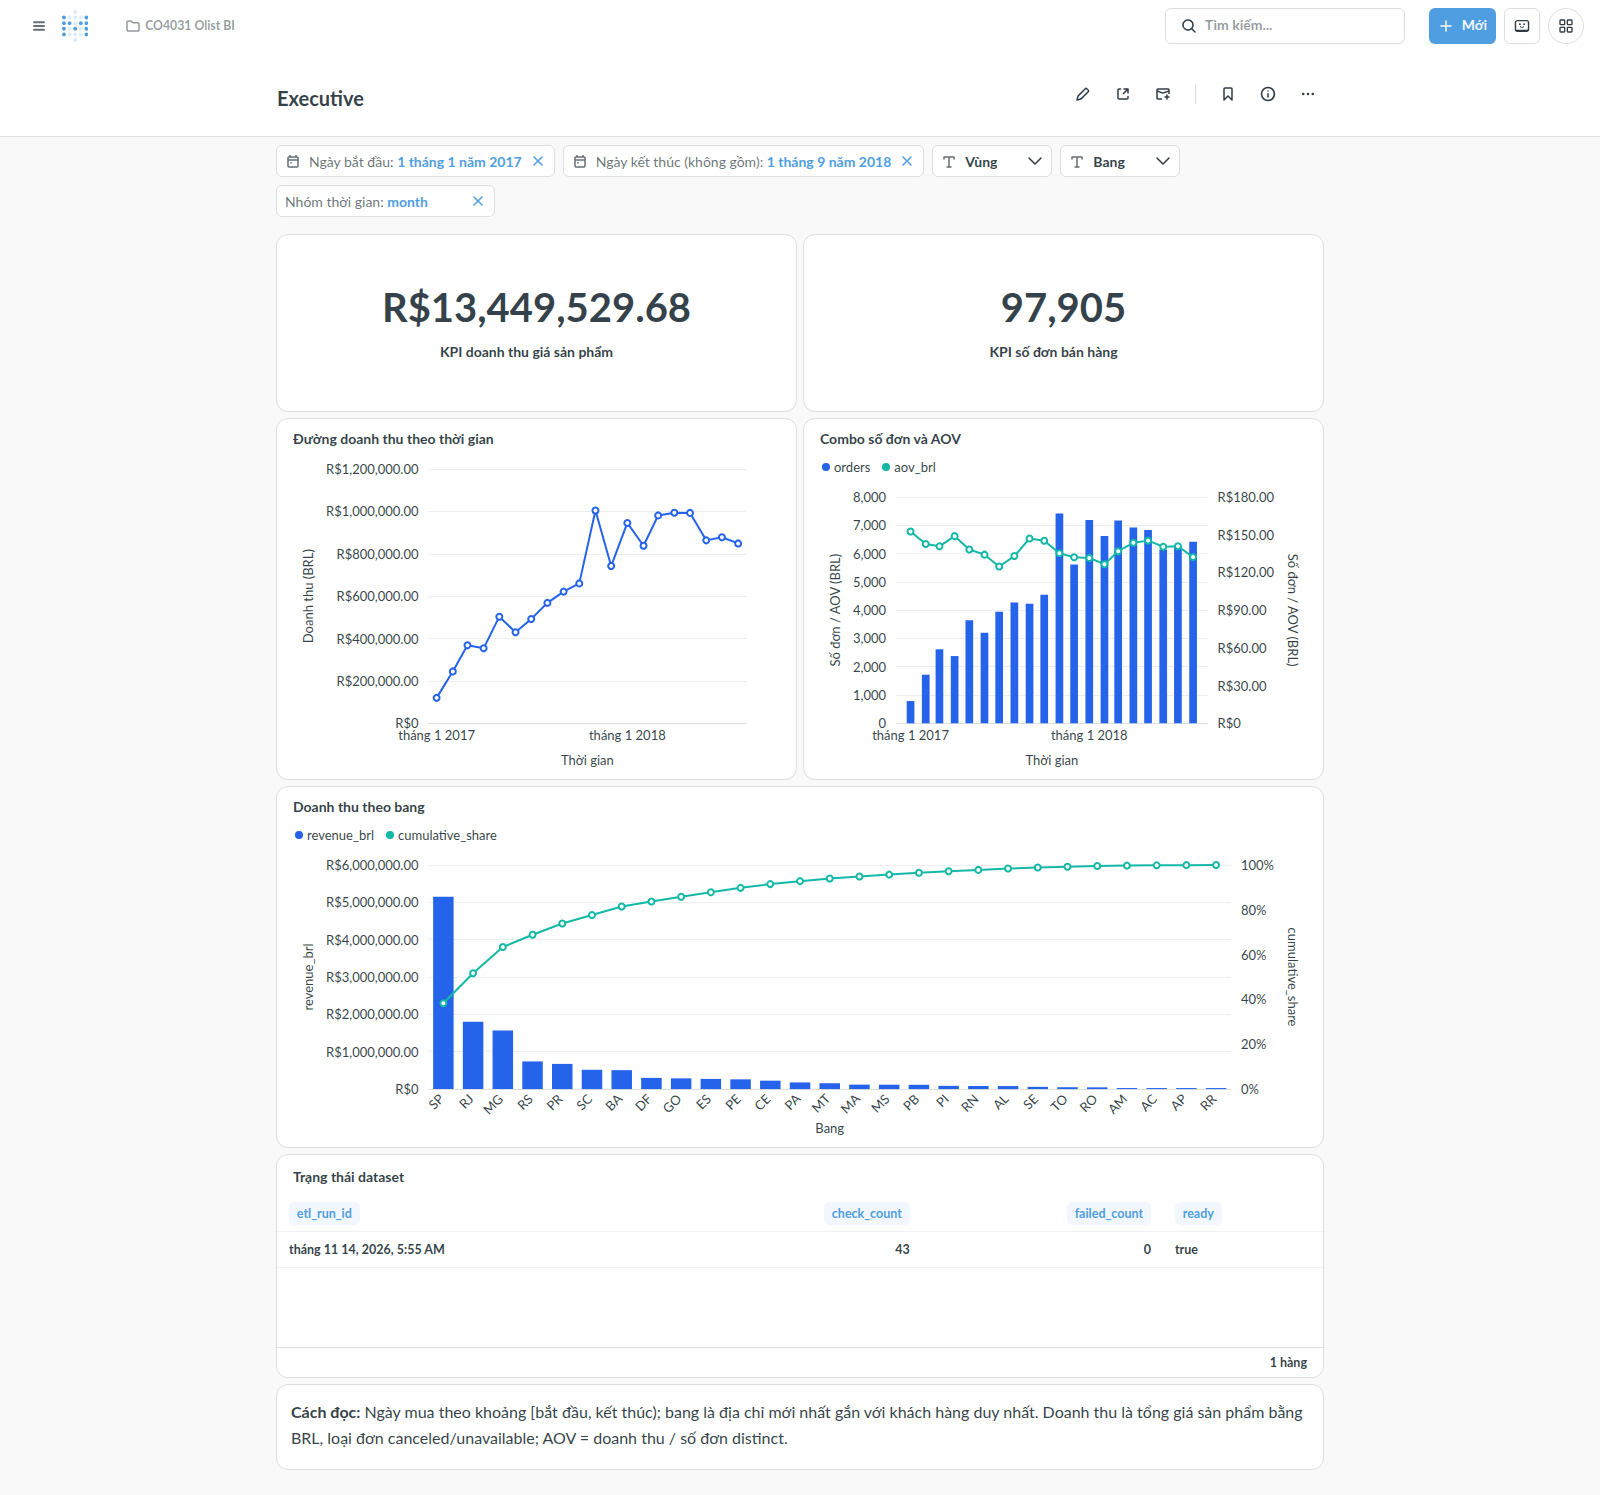
\includegraphics[height=0.74\textheight]{figures/Executive.png}\\
      {\tiny\color{muted}Dashboard Executive (lọc 01/2017 -- 08/2018)\par}
    \end{column}
  \end{columns}
\end{frame}

% =====================================================================
% CHƯƠNG 4
% =====================================================================
\setpresenter{Phan Huy Quang Minh}
\section{Mô hình cây quyết định và đánh giá rủi ro}

\begin{frame}{Tập dữ liệu, thuộc tính và cấu hình cây quyết định}
  \begin{columns}[T]
    \begin{column}{0.5\textwidth}
      \footnotesize
      \begin{itemize}
        \item \textbf{95,824 đơn} đã giao có review; nhãn: review xấu (score $\le 2$) chiếm \textbf{12.81\%}.
        \item Chia phân tầng \textbf{80/20}: 76,659 train / 19,165 test (seed 42).
        \item \textbf{Thuộc tính}: is\_late, delay\_days, delivery\_days, estimated\_days, n\_items, n\_sellers, freight\_ratio, same\_state, region (one-hot).
      \end{itemize}
      \textbf{Tiêu chí tách: information gain (entropy)}
      \vspace{-0.5em}
      \begin{align*}
        H(D) &= -\textstyle\sum_c p_c\log_2 p_c\\
        \text{Gain}(D,A) &= H(D) - \textstyle\sum_v \frac{|D_v|}{|D|}H(D_v)
      \end{align*}
      Ví dụ: tách theo is\_late: $0.5521 - 0.4793 = \mathbf{0.0728}$ bit, lớn hơn n\_sellers$>$1 (0.0068) và vùng (0.0011).
    \end{column}
    \begin{column}{0.46\textwidth}
      \footnotesize
      \begin{tabular}{@{}ll@{}}
        \toprule
        Tham số & Giá trị\\
        \midrule
        criterion & entropy\\
        max\_depth & 4 (15 lá)\\
        min\_samples\_leaf & 200\\
        class\_weight & balanced\\
        \bottomrule
      \end{tabular}\\[0.2cm]
      \textbf{Chọn độ phức tạp}: 12 cấu hình, 5-fold CV \emph{chỉ trên tập train}\\[0.05cm]
      \begin{tabular}{@{}cccc@{}}
        \toprule
        Depth & Số lá & F1 & AUC\\
        \midrule
        3 & 8 & 0.445 & 0.7307\\
        \rowcolor{accent!12}\textbf{4} & \textbf{15} & 0.426 & \textbf{0.7408}\\
        5 & 21--26 & 0.430 & 0.7436\\
        6 & 31--44 & 0.438 & 0.7456\\
        \bottomrule
      \end{tabular}\\[0.1cm]
      {\scriptsize Depth 5--6 chỉ tăng AUC thêm 0.003--0.005 nhưng số lá tăng mạnh, nên chọn depth 4 để luật dễ giải thích.\par}
    \end{column}
  \end{columns}
\end{frame}

\begin{frame}{Kết quả phân loại trên tập kiểm tra}
  \begin{columns}[T]
    \begin{column}{0.47\textwidth}
      \centering
      \footnotesize
      \textbf{Ma trận nhầm lẫn} (19,165 đơn test)\\[0.15cm]
      \renewcommand{\arraystretch}{1.5}
      \begin{tabular}{@{}l|c|c|@{}}
        \multicolumn{1}{c}{} & \multicolumn{1}{c}{Dự đoán tốt} & \multicolumn{1}{c}{Dự đoán xấu}\\
        \cline{2-3}
        Thực tế tốt & \cellcolor{good!15}13,876 (TN) & 2,835 (FP)\\
        \cline{2-3}
        Thực tế xấu & 1,061 (FN) & \cellcolor{good!15}1,393 (TP)\\
        \cline{2-3}
      \end{tabular}\\[0.35cm]
      \begin{tabular}{cccc}
        \kpi{79.67\%}{Accuracy} & \kpi{32.95\%}{Precision} & \kpi{56.76\%}{Recall} & \kpi{0.417}{F1}
      \end{tabular}\\[0.25cm]
      \begin{warnbox}
        Baseline ``luôn đoán tốt'' đạt accuracy 87.20\% nhưng \textbf{recall = 0}. Cây chấp nhận giảm accuracy để bắt được 57\% review xấu và tạo ra các phân đoạn rủi ro giải thích được.
      \end{warnbox}
    \end{column}
    \begin{column}{0.5\textwidth}
      \centering
      \begin{tikzpicture}
        \begin{axis}[bkplot, xbar, width=7.4cm, height=4.6cm, bar width=10pt,
          xmin=0, xmax=85, xlabel={Độ quan trọng (\%)}, ymajorgrids=false, xmajorgrids,
          symbolic y coords={n_sellers,delivery_days,n_items,delay_days}, ytick=data,
          yticklabels={n\_sellers,delivery\_days,n\_items,delay\_days},
          yticklabel style={font=\scriptsize},
          nodes near coords, nodes near coords style={font=\tiny},
          title={\scriptsize Feature importance của cây đã chọn}]
          \addplot[fill=bksky,draw=none] coordinates {(2.15,n_sellers)(6.89,delivery_days)(19.36,n_items)(71.60,delay_days)};
        \end{axis}
      \end{tikzpicture}\\[0.1cm]
      \footnotesize
      Nút gốc là \texttt{delay\_days} $\le 1.5$: biến liên tục mô tả mức độ trễ chi tiết hơn cờ is\_late.
    \end{column}
  \end{columns}
\end{frame}

\begin{frame}{Luật IF--THEN và xác suất theo lá}
  \begin{columns}[T]
    \begin{column}{0.54\textwidth}
      \footnotesize
      \textbf{Trích 5 trong 15 luật} \,{\scriptsize($d$: delay\_days, $t$: delivery\_days, $m$: n\_items, $v$: n\_sellers)}\\[0.1cm]
      \begin{tabular}{@{}P{4.9cm}rr@{}}
        \toprule
        IF \dots & P(xấu) & Đơn train\\
        \midrule
        $5.5 < d \le 34.5$ & \textcolor{bad}{\textbf{79.73\%}} & 2,684\\
        $4.5 < d \le 5.5$ & 64.23\% & 355\\
        $d \le 1.5,\ m > 1.5,\ v > 1.5,\ t > 11.5$ & 54.10\% & 244\\
        $d \le 1.5,\ m \le 1.5,\ t > 21.5$ & 15.23\% & 4,734\\
        $d \le 1.5,\ m \le 1.5,\ t \le 9.5$ & \textcolor{good}{\textbf{6.05\%}} & 31,480\\
        \bottomrule
      \end{tabular}\\[0.15cm]
      \textbf{Tri thức rút ra}
      \begin{enumerate}
        \item Trễ hơn khoảng 5 ngày thì rủi ro rất cao (khoảng 80\%).
        \item Đơn nhiều sản phẩm từ nhiều người bán có rủi ro 45--54\% dù không trễ (giao nhiều đợt).
        \item Không trễ nhưng giao lâu thì rủi ro vẫn tăng: 6\% lên 15\%.
      \end{enumerate}
    \end{column}
    \begin{column}{0.43\textwidth}
      \begin{keybox}[title={Xác suất theo lá (leaf rate)},coltitle=white,colbacktitle=bkblue,fonttitle=\small\bfseries]
        \texttt{class\_weight=balanced} làm \texttt{predict\_proba} lệch lên, nên hệ thống dùng \textbf{tỷ lệ review xấu thực tế của mỗi lá trên tập train}:
        \[ p_\ell = \frac{\sum_{i\in\ell} y_i}{|\ell|},\qquad E_G = \sum_{i\in G} p_{L(x_i)} \]
      \end{keybox}
      \footnotesize
      \textbf{Kiểm tra độ khớp}
      \begin{itemize}
        \item Toàn tập: kỳ vọng 12.85\%, thực tế 12.81\%.
        \item Tập test: kỳ vọng 2,497.6, thực tế 2,454 (lệch 1.8\%).
        \item \textcolor{accent}{Lưu ý}: RJ kỳ vọng 16.62\%, thực tế 18.33\%: mô hình chưa nắm hết đặc thù bang.
      \end{itemize}
    \end{column}
  \end{columns}
\end{frame}

% =====================================================================
% CHƯƠNG 5
% =====================================================================
\setpresenter{Nguyễn Minh Khánh}
\section{Hỗ trợ quyết định và tối ưu phân bổ ngân sách}

\begin{frame}{Cấu trúc DSS và các pha ra quyết định}
  \begin{columns}[T]
    \begin{column}{0.4\textwidth}
      \footnotesize
      \textbf{DSS lai}: \emph{data-driven} (OLAP trên DW) + \emph{model-driven} (cây quyết định, mô phỏng, tối ưu).\\[0.15cm]
      \begin{tikzpicture}[node distance=2mm]
        \node[dbox,minimum width=4.9cm] (d) {\textbf{Quản lý dữ liệu}: PostgreSQL DW};
        \node[dbox,below=of d,minimum width=4.9cm] (m) {\textbf{Quản lý mô hình}: tree, what-if, MILP};
        \node[dbox,below=of m,minimum width=4.9cm] (k) {\textbf{Tri thức}: 15 luật IF--THEN};
        \node[fbox,below=of k,minimum width=4.9cm] (u) {\textbf{Giao diện người dùng}: Streamlit};
      \end{tikzpicture}\\[0.15cm]
      {\scriptsize DW đảm bảo mỗi đơn chỉ có 1 review, danh mục đã chuẩn hóa và có thể truy vết. Nếu học trên dữ liệu sai grain thì nghiệm tối ưu cũng sai theo.\par}
    \end{column}
    \begin{column}{0.57\textwidth}
      \footnotesize
      \textbf{Ánh xạ các pha ra quyết định vào hệ thống}\\[0.1cm]
      \renewcommand{\arraystretch}{1.25}
      \begin{tabular}{@{}P{2.1cm}P{5.4cm}@{}}
        \toprule
        Pha & Công cụ / kết quả\\
        \midrule
        \textbf{Intelligence} & KPI, OLAP, Delivery: phát hiện RJ, đỉnh trễ 11/2017, 03/2018\\
        \textbf{Design} & Cây quyết định; biến quyết định: \% giảm đơn trễ, số ngày rút ngắn\\
        \textbf{Choice} & What-if, goal seeking, MILP, phân tích độ vững\\
        \textbf{Implementation} & Bảng phân bổ theo bang và gợi ý kiểm tra tuyến (ở mức khuyến nghị)\\
        \textbf{Evaluation} & Metrics, kiểm tra xác suất lá, độ nhạy, 43 check dữ liệu\\
        \bottomrule
      \end{tabular}
    \end{column}
  \end{columns}
\end{frame}

\begin{frame}{Phân tích what-if và độ nhạy}
  \begin{columns}[T]
    \begin{column}{0.46\textwidth}
      \footnotesize
      \textbf{Biến quyết định}: $\alpha\in[0,1]$ là tỷ lệ đơn trễ được đưa về đúng hạn; $h\in\{0..10\}$ là số ngày rút ngắn. Phạm vi: toàn quốc, bang hoặc danh mục.\\[0.1cm]
      \textbf{Lợi ích}: $B(G)=\sum_{i\in G}\big(p_{L(x_i)} - p_{L(x'_i)}\big)$\\[0.1cm]
      Đơn được sửa chọn theo một số ngẫu nhiên \textbf{cố định} (seed 42), nên các kịch bản lồng nhau và tái lập được.\\[0.15cm]
      \begin{tabular}{@{}lrr@{}}
        \toprule
        Kịch bản toàn quốc & Xấu kỳ vọng & Tránh được\\
        \midrule
        Hiện tại & 12.85\% & 0\\
        Giảm 50\% đơn trễ & 11.24\% & 1,549\\
        Giảm 100\% đơn trễ & 9.63\% & 3,085\\
        Rút ngắn 3 ngày (mọi đơn) & 11.23\% & 1,559\\
        \bottomrule
      \end{tabular}\\[0.1cm]
      {\scriptsize RJ, giảm 50\% đơn trễ: 16.62\% xuống 13.38\%, tránh được 395 review xấu.\par}
    \end{column}
    \begin{column}{0.51\textwidth}
      \centering
      \begin{tikzpicture}
        \begin{axis}[bkplot, width=7.4cm, height=4.55cm, xmin=0, xmax=100, ymin=8, ymax=18,
          xlabel={Mức giảm số đơn trễ $\alpha$ (\%)}, ylabel={Review xấu kỳ vọng (\%)},
          legend pos=north east, title={\scriptsize Độ nhạy theo mức giảm đơn trễ}]
          \addplot[bkblue,mark=*,mark size=1.3pt] coordinates {(0,12.85)(10,12.53)(25,12.04)(50,11.24)(75,10.44)(100,9.63)};
          \addlegendentry{Toàn quốc}
          \addplot[accent,mark=square*,mark size=1.3pt] coordinates {(0,16.62)(30,14.67)(50,13.38)(100,10.33)};
          \addlegendentry{RJ}
        \end{axis}
      \end{tikzpicture}\\
      \footnotesize
      Gần tuyến tính: mỗi 10\% đơn trễ được sửa làm review xấu giảm khoảng \textbf{0.32 điểm \%} trên toàn quốc và \textbf{0.63 điểm \%} tại RJ.
    \end{column}
  \end{columns}
  \vspace{0.05cm}
  {\tiny\color{muted}\hspace{0.3cm}Giả định: sau can thiệp, đơn mang rủi ro của lá mới. Đây là mô phỏng dựa trên tương quan, chưa phải tác động nhân quả đã kiểm chứng.\par}
\end{frame}

\begin{frame}{Goal seeking và xếp hạng tiềm năng cải thiện}
  \begin{columns}[T]
    \begin{column}{0.47\textwidth}
      \footnotesize
      \textbf{Goal seeking}: tìm mức $\alpha$ nhỏ nhất để đạt mục tiêu $\tau$
      \[ \alpha^* = \min\{\alpha\in\{0,0.01,\dots,1\} : R_G(\alpha) \le \tau\} \]
      \begin{tabular}{@{}lrr@{}}
        \toprule
        Mục tiêu review xấu & Cần giảm đơn trễ & Tránh được\\
        \midrule
        $\le$ 12.0\% & 27\% & 840\\
        $\le$ 11.0\% & \textbf{58\%} & 1,803\\
        $\le$ 10.0\% & 89\% & 2,751\\
        $\le$ 9.5\% & \textcolor{bad}{Không khả thi} & min 9.63\%\\
        \bottomrule
      \end{tabular}\\[0.1cm]
      {\scriptsize Tại RJ: mục tiêu 15\% cần giảm 26\% đơn trễ; mục tiêu 13\% cần giảm 57\%.\par}
    \end{column}
    \begin{column}{0.5\textwidth}
      \footnotesize
      \textbf{Tiềm năng nếu sửa hết đơn trễ} (chưa xét chi phí)\\[0.1cm]
      \begin{tabular}{@{}clrrr@{}}
        \toprule
        \# & Bang & Đơn & Tránh được & Giảm trong bang\\
        \midrule
        1 & SP & 40,271 & 805 & 2.00 điểm \%\\
        2 & RJ & 12,212 & 769 & \textbf{6.30} điểm \%\\
        3 & MG & 11,282 & 227 & 2.01 điểm \%\\
        4 & BA & 3,228 & 191 & 5.92 điểm \%\\
        5 & RS & 5,326 & 161 & 3.02 điểm \%\\
        \bottomrule
      \end{tabular}\\[0.15cm]
      \begin{warnbox}
        Xếp hạng này \textbf{chưa xét chi phí}, nên chưa thể dùng làm phương án giải ngân. Cần một mô hình chọn \emph{bang} và \emph{mức can thiệp} dưới ràng buộc ngân sách.
      \end{warnbox}
    \end{column}
  \end{columns}
\end{frame}

\begin{frame}{Mô hình tối ưu ngân sách: quy hoạch nguyên nhị phân (MILP)}
  \begin{columns}[T]
    \begin{column}{0.52\textwidth}
      \footnotesize
      24 bang (có ít nhất 100 đơn có review) $\times$ 4 mức $r\in\{25,50,75,100\%\}$, tổng cộng \textbf{96 phương án}; $x_{sr}\in\{0,1\}$.
      \begin{align*}
        \max_x\ & \textstyle\sum_{s}\sum_{r} b_{sr}\,x_{sr} &&\text{(review xấu tránh được)}\\
        \text{s.t.}\ & \textstyle\sum_r x_{sr} \le 1 \quad \forall s &&\text{(mỗi bang 1 mức)}\\
        & \textstyle\sum_{s,r} c_{sr}\,x_{sr} \le B &&\text{(ngân sách)}
      \end{align*}
      \textbf{Chi phí}: $c_{sr} = F_{sr}\cdot\gamma\cdot t_r$
      \begin{itemize}
        \item $F_{sr}$: phí ship \textbf{thật} của các đơn trễ được sửa (lấy từ DW).
        \item $\gamma=0.5$ (surcharge), $t_r = 1/1.2/1.5/2$: \textbf{giả định}, vì Olist không công bố chi phí can thiệp.
      \end{itemize}
      {\scriptsize Giải bằng SciPy \texttt{milp} + HiGHS, mỗi bài toán 0.03--0.06 s. Greedy nâng cấp dần theo lợi ích/chi phí cận biên làm đối chứng.\par}
    \end{column}
    \begin{column}{0.45\textwidth}
      \centering
      \footnotesize
      \textbf{MILP so với greedy}\\[0.05cm]
      \begin{tabular}{@{}rcrrr@{}}
        \toprule
        Ngân sách & Bang & MILP & Greedy & Chênh\\
        \midrule
        5,000 & 2 & 226.1 & 225.6 & 0.24\%\\
        10,000 & 5 & 448.2 & 446.6 & 0.36\%\\
        20,000 & 12 & 817.5 & 817.5 & 0.00\%\\
        \rowcolor{accent!12}40,000 & 19 & 1,410.9 & 1,405.1 & 0.41\%\\
        80,000 & 22 & 2,194.7 & 2,194.3 & 0.02\%\\
        160,000 & 24 & 3,079.8 & 3,078.2 & 0.05\%\\
        \bottomrule
      \end{tabular}\\[0.15cm]
      \begin{keybox}
        Lợi ích giảm dần theo ngân sách: tăng từ 80k lên 160k BRL chỉ tránh thêm khoảng 885 review xấu. Greedy gần tối ưu ở các mốc này (chênh $\le$ 0.41\%), nhưng chỉ MILP \textbf{đảm bảo} nghiệm tối ưu.
      \end{keybox}
    \end{column}
  \end{columns}
\end{frame}

\begin{frame}{Kết quả tại 40,000 BRL và độ nhạy theo chi phí}
  \centering
  \begin{tabular}{@{}c@{\hspace{1.4cm}}c@{\hspace{1.4cm}}c@{\hspace{1.4cm}}c@{}}
    \kpi{1,411}{review xấu tránh được} & \kpi{12.85\%\,$\to$\,11.38\%}{review xấu kỳ vọng toàn quốc} & \kpi{19}{bang được chọn} & \kpi{39,966 BRL}{chi phí, sửa 2,893 đơn trễ}
  \end{tabular}\\[0.3cm]
  \raggedright
  \begin{columns}[T]
    \begin{column}{0.47\textwidth}
      \footnotesize
      \textbf{Phương án tối ưu (chi phí mặc định)}
      \begin{itemize}
        \item \textbf{Giảm 50\% đơn trễ}: RJ, SP, MG, BA, RS, SC, ES, PR, GO, DF, PI, MS
        \item \textbf{Giảm 25\% đơn trễ}: CE, PE, PA, MT, AL, SE, TO
      \end{itemize}
      \vspace{0.1cm}
      \begin{keybox}
        Nhân $\gamma$ và $B$ cùng tỷ lệ thì nghiệm \textbf{không đổi} (đã có test). Chỉ hệ số tier $t_r$ mới làm thay đổi cấu trúc nghiệm.
      \end{keybox}
    \end{column}
    \begin{column}{0.49\textwidth}
      \footnotesize
      \textbf{Độ nhạy theo hệ số tier} (ngân sách 40,000 BRL)\\[0.1cm]
      \setlength{\tabcolsep}{4pt}
      \begin{tabular}{@{}llrrr@{}}
        \toprule
        Tier & 25/50/75/100\% & Tránh được & Bang & Đơn sửa\\
        \midrule
        Phẳng & 1/1/1/1 & 1,818.4 & 8 & 3,737\\
        \rowcolor{accent!12}Mặc định & 1/1.2/1.5/2 & 1,410.9 & 19 & 2,893\\
        Dốc & 1/1.5/2.25/3.5 & 1,240.6 & 20 & 2,525\\
        \bottomrule
      \end{tabular}\\[0.1cm]
      Tier \textbf{phẳng}: sửa \emph{sâu} ở ít bang. Tier \textbf{dốc}: sửa \emph{nhẹ} ở nhiều bang.\\[0.1cm]
      \begin{warnbox}
        Cấu trúc chi phí thay đổi thì phương án thay đổi. Thu thập báo giá thật quan trọng hơn tinh chỉnh bộ giải, nên cần kiểm tra \textbf{độ vững} của khuyến nghị.
      \end{warnbox}
    \end{column}
  \end{columns}
\end{frame}

\begin{frame}{Độ vững của khuyến nghị: câu trả lời cho bài toán quyết định}
  \begin{columns}[T]
    \begin{column}{0.56\textwidth}
      \footnotesize
      \textbf{Thiết kế}: 2 cơ chế chi phí (phí ship thật / đồng đều) $\times$ 3 tier = \textbf{6 bộ giả định}, giải ở 3 mức ngân sách 10k / 20k / 40k BRL, tổng cộng \textbf{18 bài toán}.\\
      Bang thuộc \emph{ưu tiên k} nếu ở mức ngân sách thứ k nó được chọn trong ít nhất \textbf{4/6} bộ giả định.\\[0.15cm]
      \renewcommand{\arraystretch}{1.2}
      \begin{tabular}{@{}lP{6.2cm}@{}}
        \toprule
        Ưu tiên & Bang (số bộ giả định chọn ở 10k/20k/40k)\\
        \midrule
        \textcolor{accent}{\textbf{1 (10k)}} & \textbf{RJ} (5/5/6), \textbf{GO} (4/5/6), \textbf{PR} (4/4/6), \textbf{RN} (5/4/4)\\
        2 (20k) & RS, ES, SP, SE, PA, SC, AL, TO, MT, DF, MG\\
        3 (40k) & BA, PI, MS, PE, CE\\
        Ít chọn & RO, PB, MA, AM\\
        \bottomrule
      \end{tabular}\\[0.1cm]
      {\scriptsize RJ được chọn 16/18 lần. SP có tiềm năng tuyệt đối lớn nhất nhưng chỉ ổn định từ 20k: số review xấu tránh được nhiều chưa chắc là lựa chọn vững.\par}
    \end{column}
    \begin{column}{0.41\textwidth}
      \begin{keybox}[title={Đề xuất quản lý},coltitle=white,colbacktitle=bkblue,fonttitle=\small\bfseries]
        \begin{enumerate}\setlength{\itemsep}{1pt}
          \item Ưu tiên điều tra \textbf{RJ} và nhóm \textbf{GO / PR / RN}: tuyến, người bán, hãng vận chuyển.
          \item Thu thập \textbf{báo giá thật} theo tuyến rồi giải lại mô hình.
          \item \textbf{Thử nghiệm có đối chứng} trên một nhóm tuyến trước khi mở rộng.
          \item Xử lý trải nghiệm \textbf{đơn nhiều người bán} (gom hàng, thông báo giao nhiều đợt).
        \end{enumerate}
      \end{keybox}
      {\scriptsize Mức can thiệp cụ thể còn dao động (RJ từ 25\% đến 100\% tùy kịch bản), nên khuyến nghị nêu bang ưu tiên kèm điều kiện chi phí.\par}
    \end{column}
  \end{columns}
\end{frame}

% =====================================================================
% CHƯƠNG 6
% =====================================================================
\setpresenter{Nguyễn Minh Khánh}
\section{Kết luận và hướng phát triển}

\begin{frame}{Đối chiếu với yêu cầu của bài tập lớn}
  \centering
  \footnotesize
  \renewcommand{\arraystretch}{1.28}
  \begin{tabular}{@{}c P{4.2cm} P{7.6cm} c@{}}
    \toprule
    & \textbf{Yêu cầu} & \textbf{Hiện thực trong đề tài} & \textbf{Chương}\\
    \midrule
    \textcolor{good}{\checkmark} & Phân tích yêu cầu, bài toán cụ thể & Bài toán phân bổ ngân sách giảm review xấu trên dữ liệu Olist 99k đơn; yêu cầu phân tích và hỗ trợ quyết định & 1\\
    \textcolor{good}{\checkmark} & DW đa chiều + ETL & Fact constellation (2 fact, 4 dimension dùng chung); ETL Python + SQL, 43 checks, metadata, lineage & 2\\
    \textcolor{good}{\checkmark} & Backend + frontend & PostgreSQL ROLAP, partition, 3 MV, 5 phép toán OLAP; Streamlit 5 trang, Metabase 3 dashboard & 2--3\\
    \textcolor{good}{\checkmark} & DSS dựa trên DW & Cây quyết định entropy, what-if, độ nhạy, goal seeking, MILP, phân tích độ vững & 4--5\\
    \textcolor{good}{\checkmark} & Đánh giá, hạn chế, hướng phát triển & Đánh giá 3 lớp: chất lượng dữ liệu, chất lượng mô hình, chất lượng phương án; pytest + đối soát BI & 4--6\\
    \textcolor{good}{\checkmark} & Nộp bài & Báo cáo PDF, mã nguồn \texttt{src/} trên GitHub, dữ liệu \texttt{data/}, slide PDF & --\\
    \bottomrule
  \end{tabular}
\end{frame}

\begin{frame}{Kết luận, hạn chế và hướng phát triển}
  \begin{columns}[T]
    \begin{column}{0.32\textwidth}
      \begin{tcolorbox}[enhanced,colback=good!6,colframe=good,boxrule=0pt,toprule=2.5pt,arc=1pt,fontupper=\scriptsize,title={Kết quả đạt được},coltitle=good,colbacktitle=good!6,fonttitle=\small\bfseries,height=6.3cm]
        \begin{itemize}\setlength{\itemsep}{2pt}
          \item Hệ thống hoàn chỉnh từ CSV đến DW, OLAP, dashboard và DSS; tái lập được bằng vài lệnh.
          \item 40k BRL: tránh khoảng \textbf{1,411} review xấu (12.85\% xuống 11.38\%).
          \item Nhóm ưu tiên vững: \textbf{RJ, GO, PR, RN}.
          \item Khuyến nghị đi kèm điều kiện chi phí, không chỉ là một thứ hạng.
        \end{itemize}
      \end{tcolorbox}
    \end{column}
    \begin{column}{0.32\textwidth}
      \begin{tcolorbox}[enhanced,colback=accent!6,colframe=accent,boxrule=0pt,toprule=2.5pt,arc=1pt,fontupper=\scriptsize,title={Hạn chế},coltitle=accent,colbacktitle=accent!6,fonttitle=\small\bfseries,height=6.3cm]
        \begin{itemize}\setlength{\itemsep}{2pt}
          \item Chi phí can thiệp là \textbf{giả định} (surcharge, tier).
          \item Quan hệ trễ và review xấu là \textbf{tương quan}, lợi ích chưa kiểm chứng thực tế.
          \item Thuộc tính chỉ có sau khi giao, nên mô hình không dùng để cảnh báo sớm.
          \item Chia train/test ngẫu nhiên; không dùng mã bang (RJ lệch 1.7 điểm \%).
          \item Full refresh, chưa có SCD type 2.
        \end{itemize}
      \end{tcolorbox}
    \end{column}
    \begin{column}{0.32\textwidth}
      \begin{tcolorbox}[enhanced,colback=bksky!6,colframe=bksky,boxrule=0pt,toprule=2.5pt,arc=1pt,fontupper=\scriptsize,title={Hướng phát triển},coltitle=bkblue,colbacktitle=bksky!6,fonttitle=\small\bfseries,height=6.3cm]
        \begin{itemize}\setlength{\itemsep}{2pt}
          \item Báo giá thật theo tuyến, ràng buộc công suất; tối ưu theo tuyến.
          \item Thử nghiệm A/B để kiểm chứng lợi ích.
          \item Đánh giá theo thời gian, calibration, khoảng bất định.
          \item Khai thác review text, geolocation (khoảng cách), ngày lễ.
          \item Incremental ETL, SCD type 2, lập lịch, triển khai cloud.
        \end{itemize}
      \end{tcolorbox}
    \end{column}
  \end{columns}
\end{frame}

% =====================================================================
% CẢM ƠN & Q&A
% =====================================================================
\begin{frame}[plain,noframenumbering]
  \begin{tikzpicture}[remember picture,overlay]
    \fill[bkblue] (current page.north west) rectangle (current page.south east);
    \fill[accent] ([yshift=-0.9cm]current page.west) rectangle ([yshift=-0.98cm]current page.east);
    \node[text=white,font=\fontsize{34}{36}\selectfont\bfseries] at ([yshift=1.3cm]current page.center) {Cảm ơn thầy và các bạn};
    \node[text=white!80!bkblue,font=\Large] at ([yshift=0.1cm]current page.center) {đã lắng nghe!};
    \node[text=white,font=\fontsize{26}{28}\selectfont\bfseries] at ([yshift=-2.0cm]current page.center) {Hỏi \& Đáp};
    \node[text=white!70!bkblue,font=\scriptsize] at ([yshift=-3.3cm]current page.center)
      {\texttt{github.com/taita2005/co4031-olist-dw-dss}\quad$\cdot$\quad Nhóm 02 -- L01 \quad$\cdot$\quad CO4031 -- HK261};
  \end{tikzpicture}
\end{frame}

\end{document}
